% 放在介绍CTC折叠映射B的段落之后、最优路径公式之前。
% 配图为教学构造示例，不是附件样本的实测结果。
图~\ref{fig:p1_ctc_principle}以给定词 \texttt{HELLO} 为例说明CTC路径与词时间区间的关系。
一条合法路径可以在多个连续时刻重复输出同一字符，也可以包含空白符。
折叠时，先合并相邻的重复符号，再删除空白符，得到与给定转写一致的字符序列。
例如，两组字母 \texttt{L} 之间存在空白符，因而不会被合并为同一个字母；
删除空白符后仍保留两个 \texttt{L}。
强制对齐进一步保留各字符对应的原始时间位置，以首个文字字符的起点和末个文字字符的终点确定词区间。

\begin{figure}[htbp]
    \centering
    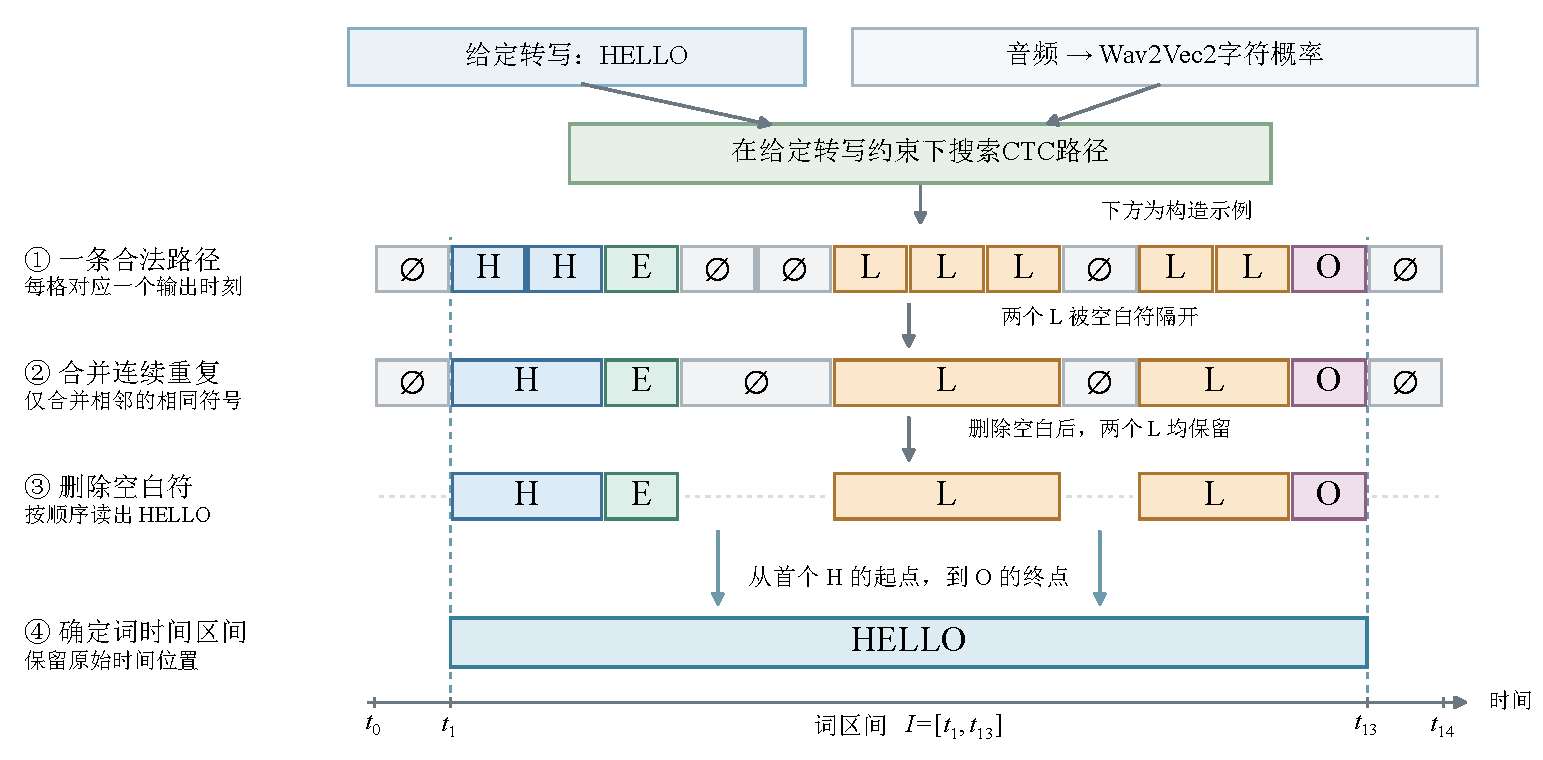
\includegraphics[width=\textwidth]{figures/fig_5_4_ctc_principle.pdf}
    \caption{CTC路径折叠与词级时间定位示意。
    示例路径经合并连续重复符号、删除空白符后得到给定词 \texttt{HELLO}，
    其候选时间区间为 $[t_1,t_{13}]$。
    字符位置与时间刻度为教学构造，不代表实测对齐结果。}
    \label{fig:p1_ctc_principle}
\end{figure}

图中仅展示一条满足转写约束的路径。实际计算时，本文利用音频的字符概率，
在所有与给定转写一致的合法路径中搜索概率最大的路径，再由该路径估计各词的时间边界。
